\documentclass[xcolor=table, 11pt, aspectratio=169]{beamer}

%\usepackage{arev}
\usepackage{amsmath,amssymb,amscd}
\usepackage{dsfont}
\usepackage{mathrsfs}
\usepackage{yfonts}
\usepackage{bm}
\usepackage{graphicx}
\usepackage{tabularx}
\usepackage{animate}
\usepackage{listings}
\usepackage{pifont}
%\usepackage{mathtools}
%\usepackage{ifthen}

%\usepackage{xeCJK}
%\usepackage{fontspec}
%\newfontfamily\cjkfont{PingFang SC}
%\setCJKmainfont{PingFang SC}
\newcolumntype{x}{>{\centering\arraybackslash}X}
\renewcommand{\arraystretch}{1.5}
\newcommand{\uone}{\mathrm U(1)}
\DeclareMathOperator{\img}{img}
\lstset{language=GAP}

\usepackage{tikz}
	\usetikzlibrary{calc}
	\usetikzlibrary{arrows,shapes, positioning, matrix}
	\usetikzlibrary{decorations.markings}
	\tikzset{>=stealth}
	\tikzstyle arrowstyle=[scale=1]
	\tikzstyle directed=[postaction={decorate,decoration={markings,
 	   mark=at position .15 with {\arrow[arrowstyle]{stealth}}}}]
\tikzstyle string=[thick,postaction={decorate,decoration={markings,
    mark=at position .55 with {\arrow[arrowstyle]{stealth}}}}]
\tikzstyle dual_string=[dashed,postaction={decorate,decoration={markings,
    mark=at position .55 with {\arrow[arrowstyle]{stealth}}}}]

\tikzstyle dw=[thick,postaction={decorate,decoration={markings,
    mark=at position 1 with {\arrow[arrowstyle]{stealth}}}}]
\tikzstyle group=[mbg]
\newcommand*{\halfway}{0.5*\pgfdecoratedpathlength+.5*8pt}\tikzstyle arrowstyle=[scale=1]
\newcommand*{\halfwayb}{0.5*\pgfdecoratedpathlength}
\tikzstyle arrowstyle=[scale=1]
\tikzstyle fermion=[thick,postaction={decorate},decoration={markings,
    mark=at position \halfway with {\arrow[arrowstyle]{latex}}}]
\tikzstyle fermion2=[thick,postaction={decorate},decoration={markings,
        mark=at position \halfwayb with {\arrow[arrowstyle]{latex}}}]

\usepackage{pgffor}
\newcommand{\mb}[1]{\mathbf{#1}}
\renewcommand{\cal}[1]{\mathcal{#1}}

\newcommand{\ag}[2]{#1_\mb{#2}}
\newcommand{\cohosub}[1]{\scalebox{0.72}{\textswab{#1}}}
\newcommand{\cohosubsub}[1]{\scalebox{0.6}{\textswab{#1}}}
\newcommand{\coho}[1]{\textswab{#1}}

\DeclareMathOperator{\tr}{Tr}
\DeclareMathOperator{\im}{Im}
\DeclareMathOperator{\re}{Re}

\mode<presentation>
{
  %\usetheme{Warsaw}
  % or ...
  %\useoutertheme{rectangle}
  \setbeamertemplate{frametitle}[default][center]
  \defbeamertemplate{itemize item}{flat}{\begin{pgfpicture}{-1ex}{0ex}{1ex}{2ex}
      \pgfpathcircle{\pgfpoint{0pt}{.6ex}}{0.6ex}
      \pgfusepath{fill}
    \end{pgfpicture}%
  }
  \defbeamertemplate{itemize subitem}{flat}{\footnotesize\raise0.5pt\hbox{\textbullet}}
  \defbeamertemplate{itemize subsubitem}{flat}{\footnotesize\raise0.5pt\hbox{\textbullet}}

  %\useinnertheme{circles}
  \setbeamertemplate{items}[flat]
  \setbeamertemplate{sections/subsections in toc}[circle]
  \setbeamertemplate{blocks}[rounded]
  \setbeamertemplate{title page}[default][colsep=-4bp,rounded=true]
  \setbeamertemplate{part page}[default][colsep=-4bp,rounded=true]
  \setbeamercovered{transparent}
  %\usecolortheme{spruce}
  %\definecolor{THU}{RGB}{116,61,130}
  \definecolor{mbg}{RGB}{0,0,160}
  \setbeamercolor*{palette primary}{fg=white,bg=mbg}
  \setbeamercolor*{titlelike}{parent=palette primary}
  \setbeamercolor*{structure}{fg=mbg}
  \setbeamercolor{frametitle}{fg=white,bg=mbg}
  % or whatever (possibly just delete it)
  \setbeamercolor{block title}{bg=mbg,fg=white}
  \setbeamercolor{block body}{bg=mbg!15}


  \addtobeamertemplate{navigation symbols}{}{ \hspace{1em}%
    \usebeamerfont{footline}%
    \insertframenumber / \inserttotalframenumber }
}


%\usepackage[english]{babel}
% or whatever

%\usepackage[latin1]{inputenc}
% or whatever

%\usepackage{times}
%\usepackage[T1]{fontenc}
% Or whatever. Note that the encoding and the font should match. If T1
% does not look nice, try deleting the line with the fontenc.

\title[Space-group SPTs] % (optional, use only with long paper titles)
{Classification of Topological Crystalline States}

\author[Y Qi] % (optional, use only with lots of authors)
{Yang~Qi}
% - Give the names in the same order as the appear in the paper.
% - Use the \inst{?} command only if the authors have different
%   affiliation.

\institute[Fudan] % (optional, but mostly needed)
{Department of Physics, Fudan University}
% - Use the \inst command only if there are several affiliations.
% - Keep it simple, no one is interested in your street address.

%\date{2016 Annual Meeting of Fudan CFTPP} % (optional, should be abbreviation of conference name)
\date{WENG, Xi'an, April 2024.}
% - Either use conference name or its abbreviation.
% - Not really informative to the audience, more for people (including
%   yourself) who are reading the slides online

\subject{Theoretical Physics}
% This is only inserted into the PDF information catalog. Can be left
% out.



% If you have a file called "university-logo-filename.xxx", where xxx
% is a graphic format that can be processed by latex or pdflatex,
% resp., then you can add a logo as follows:

\pgfdeclareimage[height=1cm]{university-logo}{../resources/fudan}
\logo{\pgfuseimage{university-logo}}

\AtBeginSection[]
{
\begin{frame}{Outline}
%	\begin{columns}
%		\begin{column}[t]{.45\textwidth}
%		\begin{center}
%			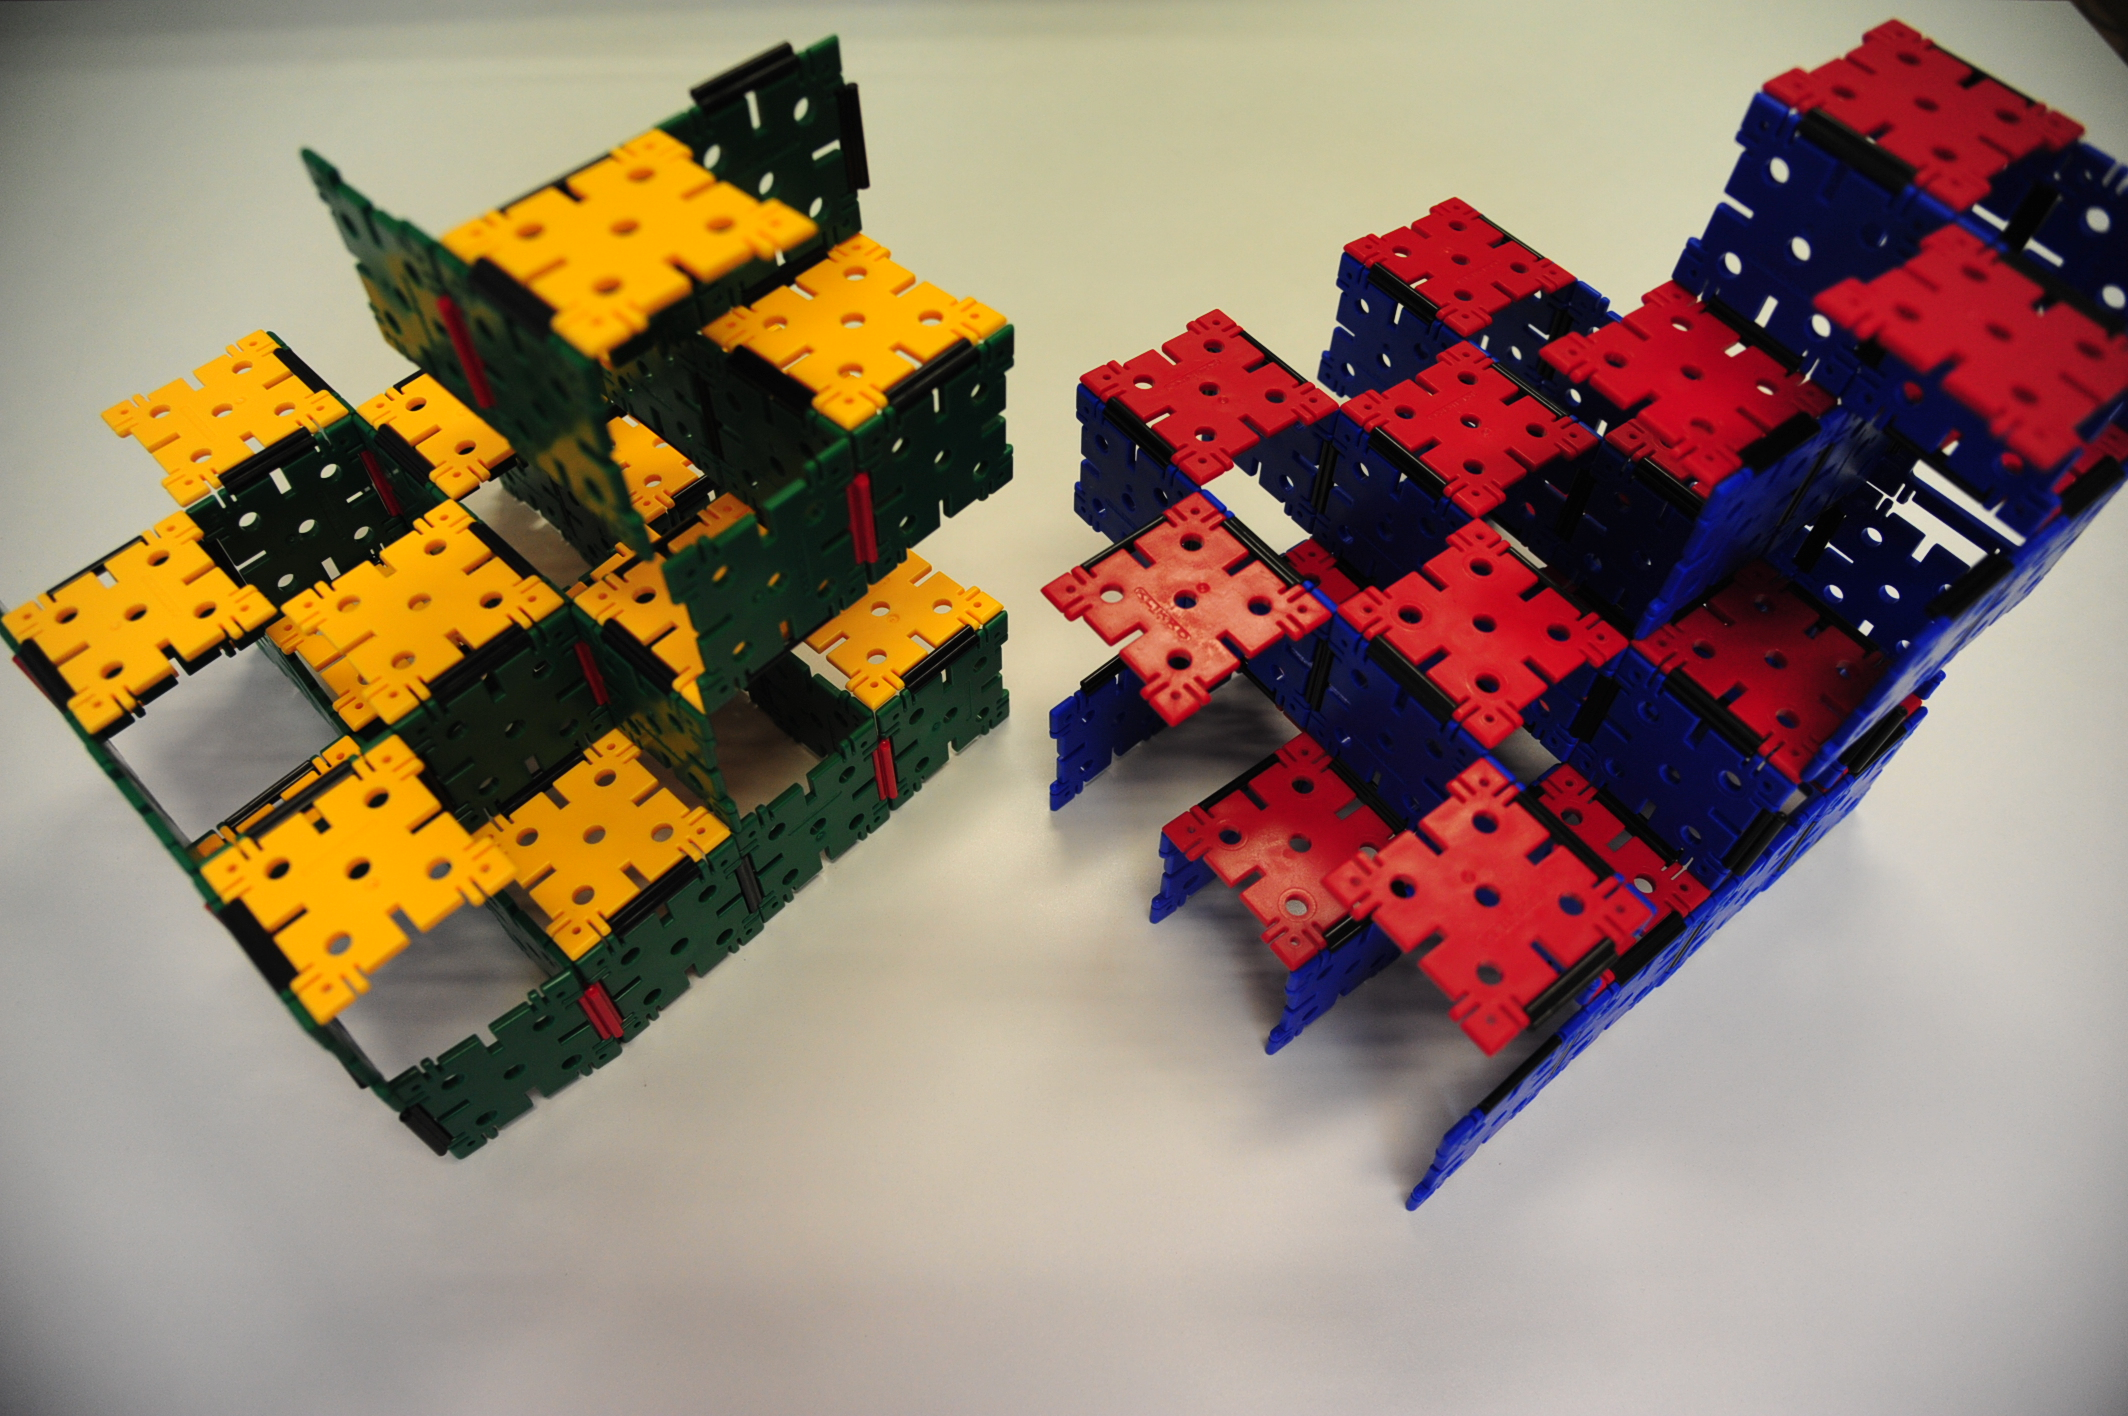
\includegraphics[height=4cm]{toys}
%		\end{center}
%	\end{column}
%	\begin{minipage}[t][0.5\textheight]{0.55\textwidth}
      \tableofcontents[currentsection]
%    \end{minipage}\hfill
%	\end{columns}
\end{frame}
}


% Delete this, if you do not want the table of contents to pop up at
% the beginning of each subsection:

\begin{document}

\begin{frame}
  \titlepage
\end{frame}

\begin{frame}{Collaborators}
  \begin{itemize}
  \item Tian Yuan: Fudan University.
  \item Chen Fang: Institute of Physics, CAS.
\end{itemize}
\vspace{4em}
\begin{center}
        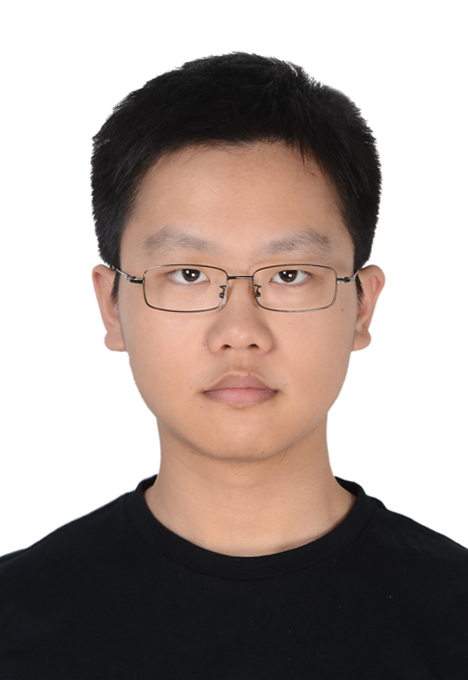
\includegraphics[height=3.5cm]{../people/tianyuan}~~~~
      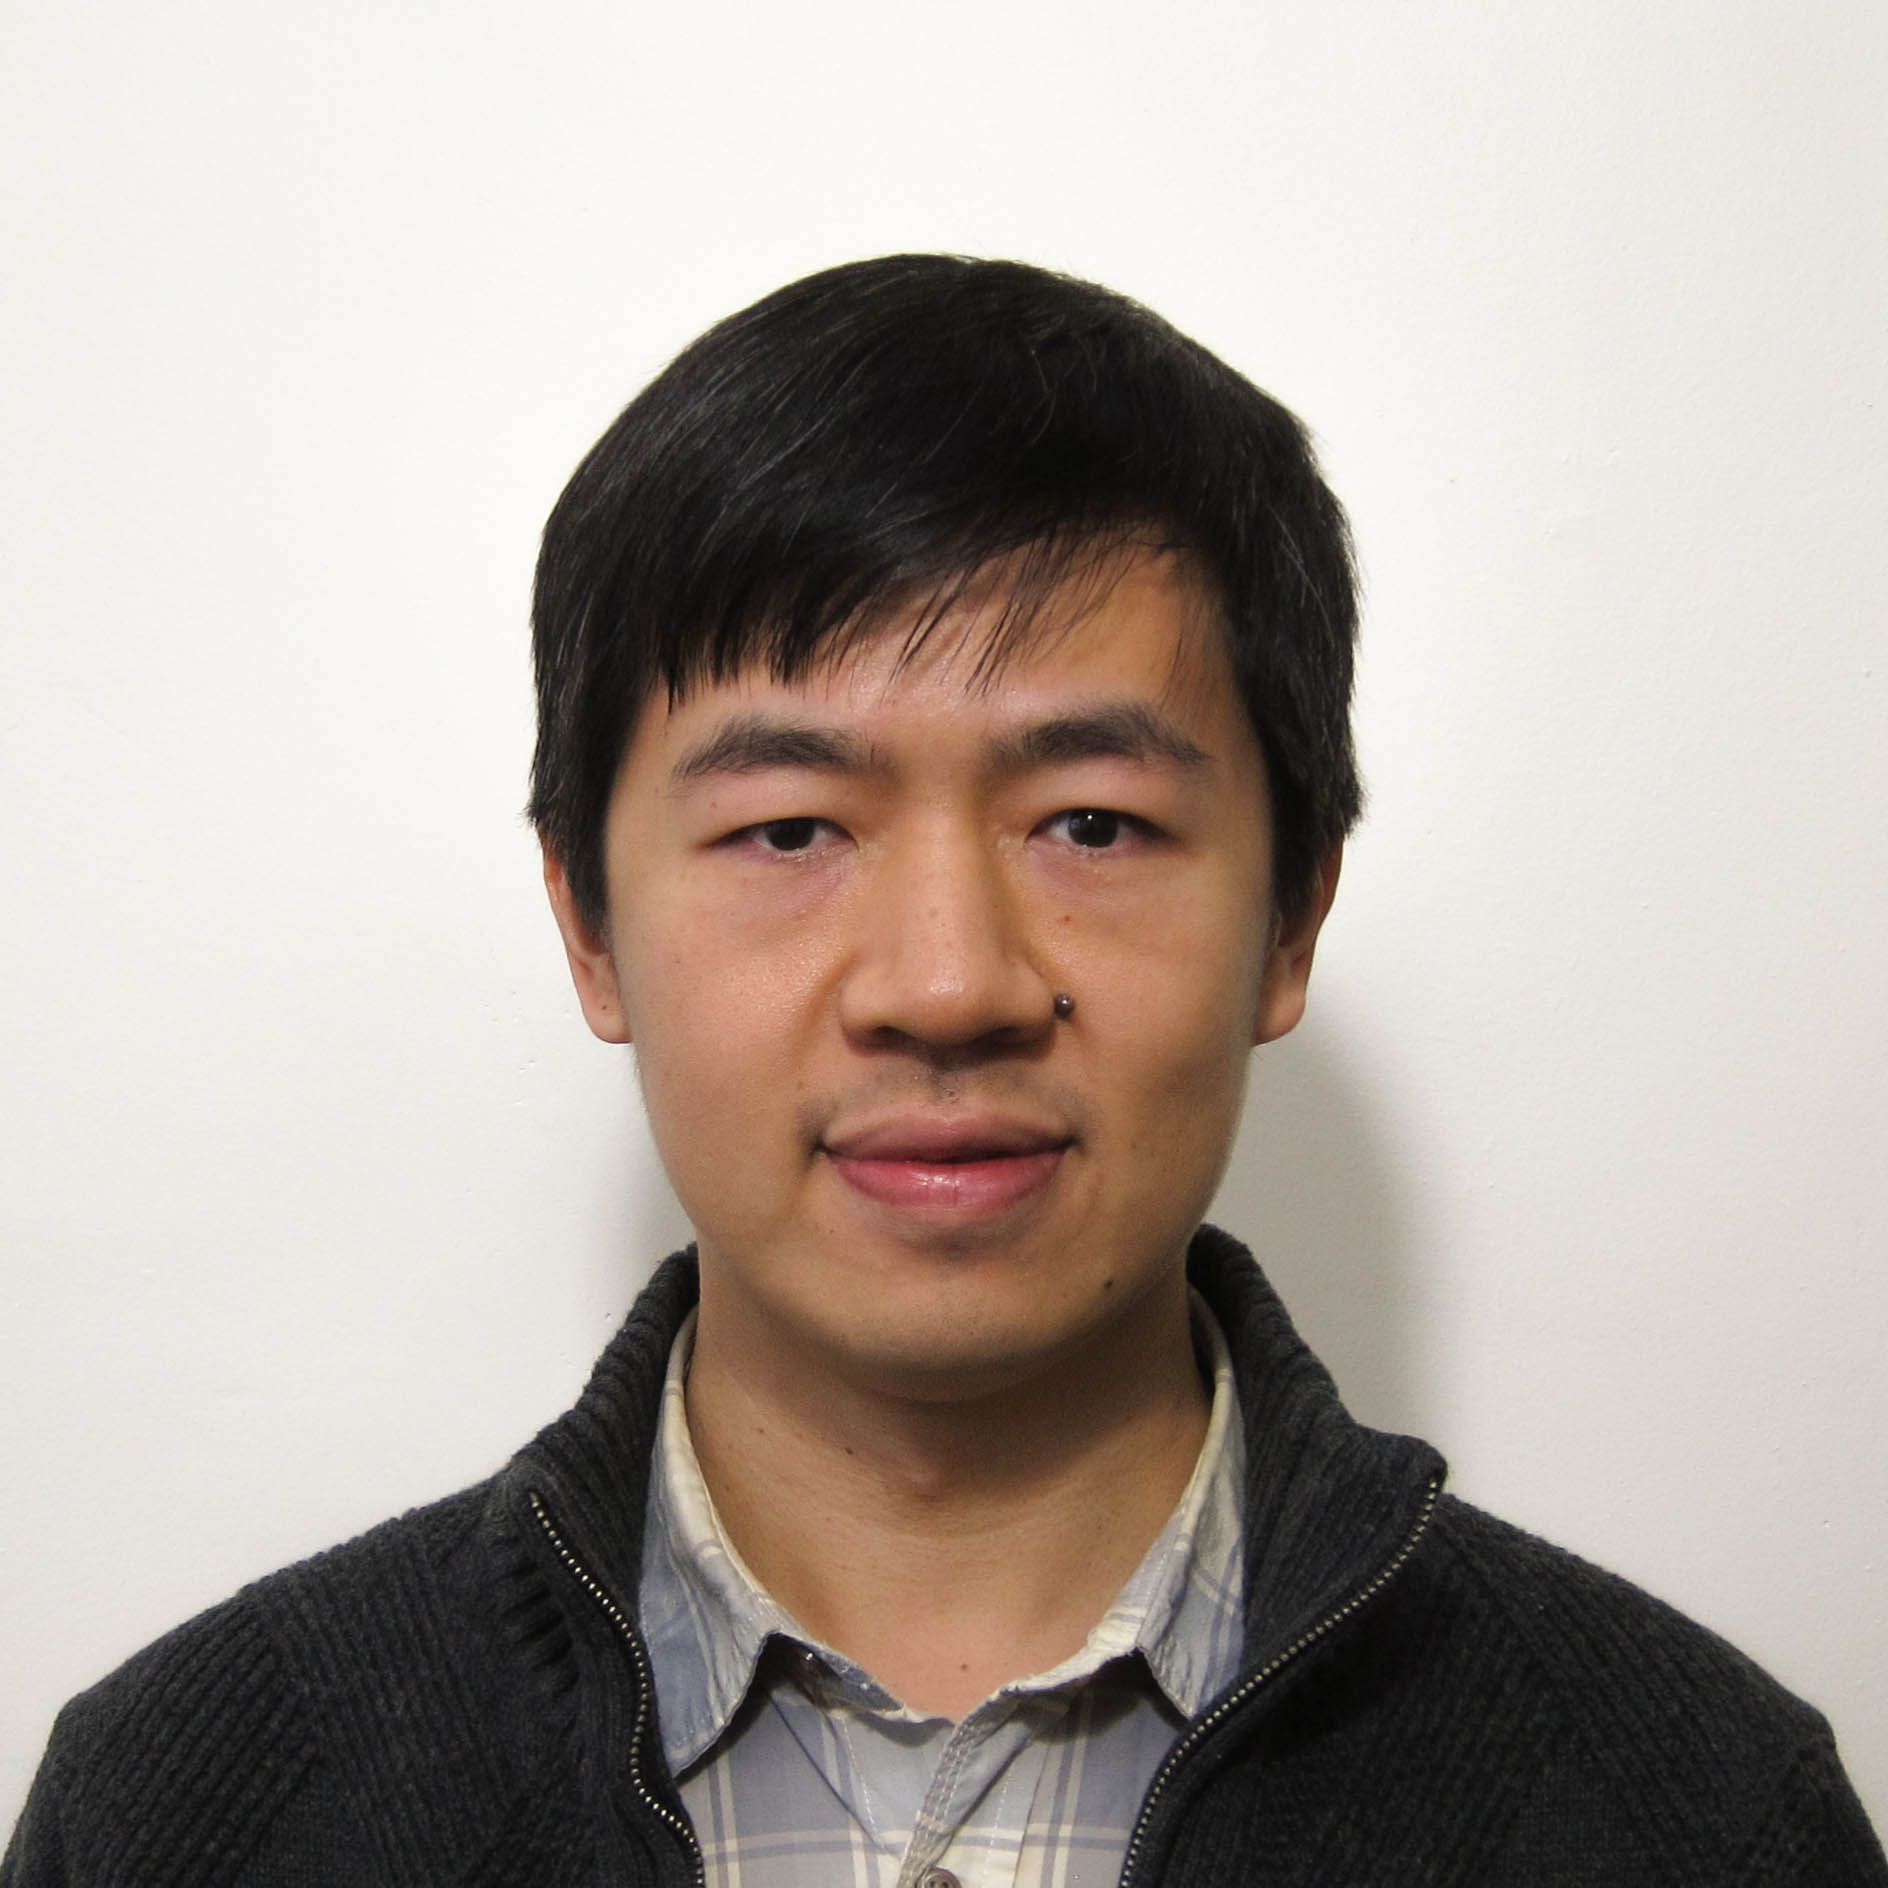
\includegraphics[height=3.5cm]{../people/chenfang}
    \end{center}
\end{frame}

\begin{frame}{Outline}
%	\begin{columns}
%		\begin{column}[t]{.45\textwidth}
%		\begin{center}
%			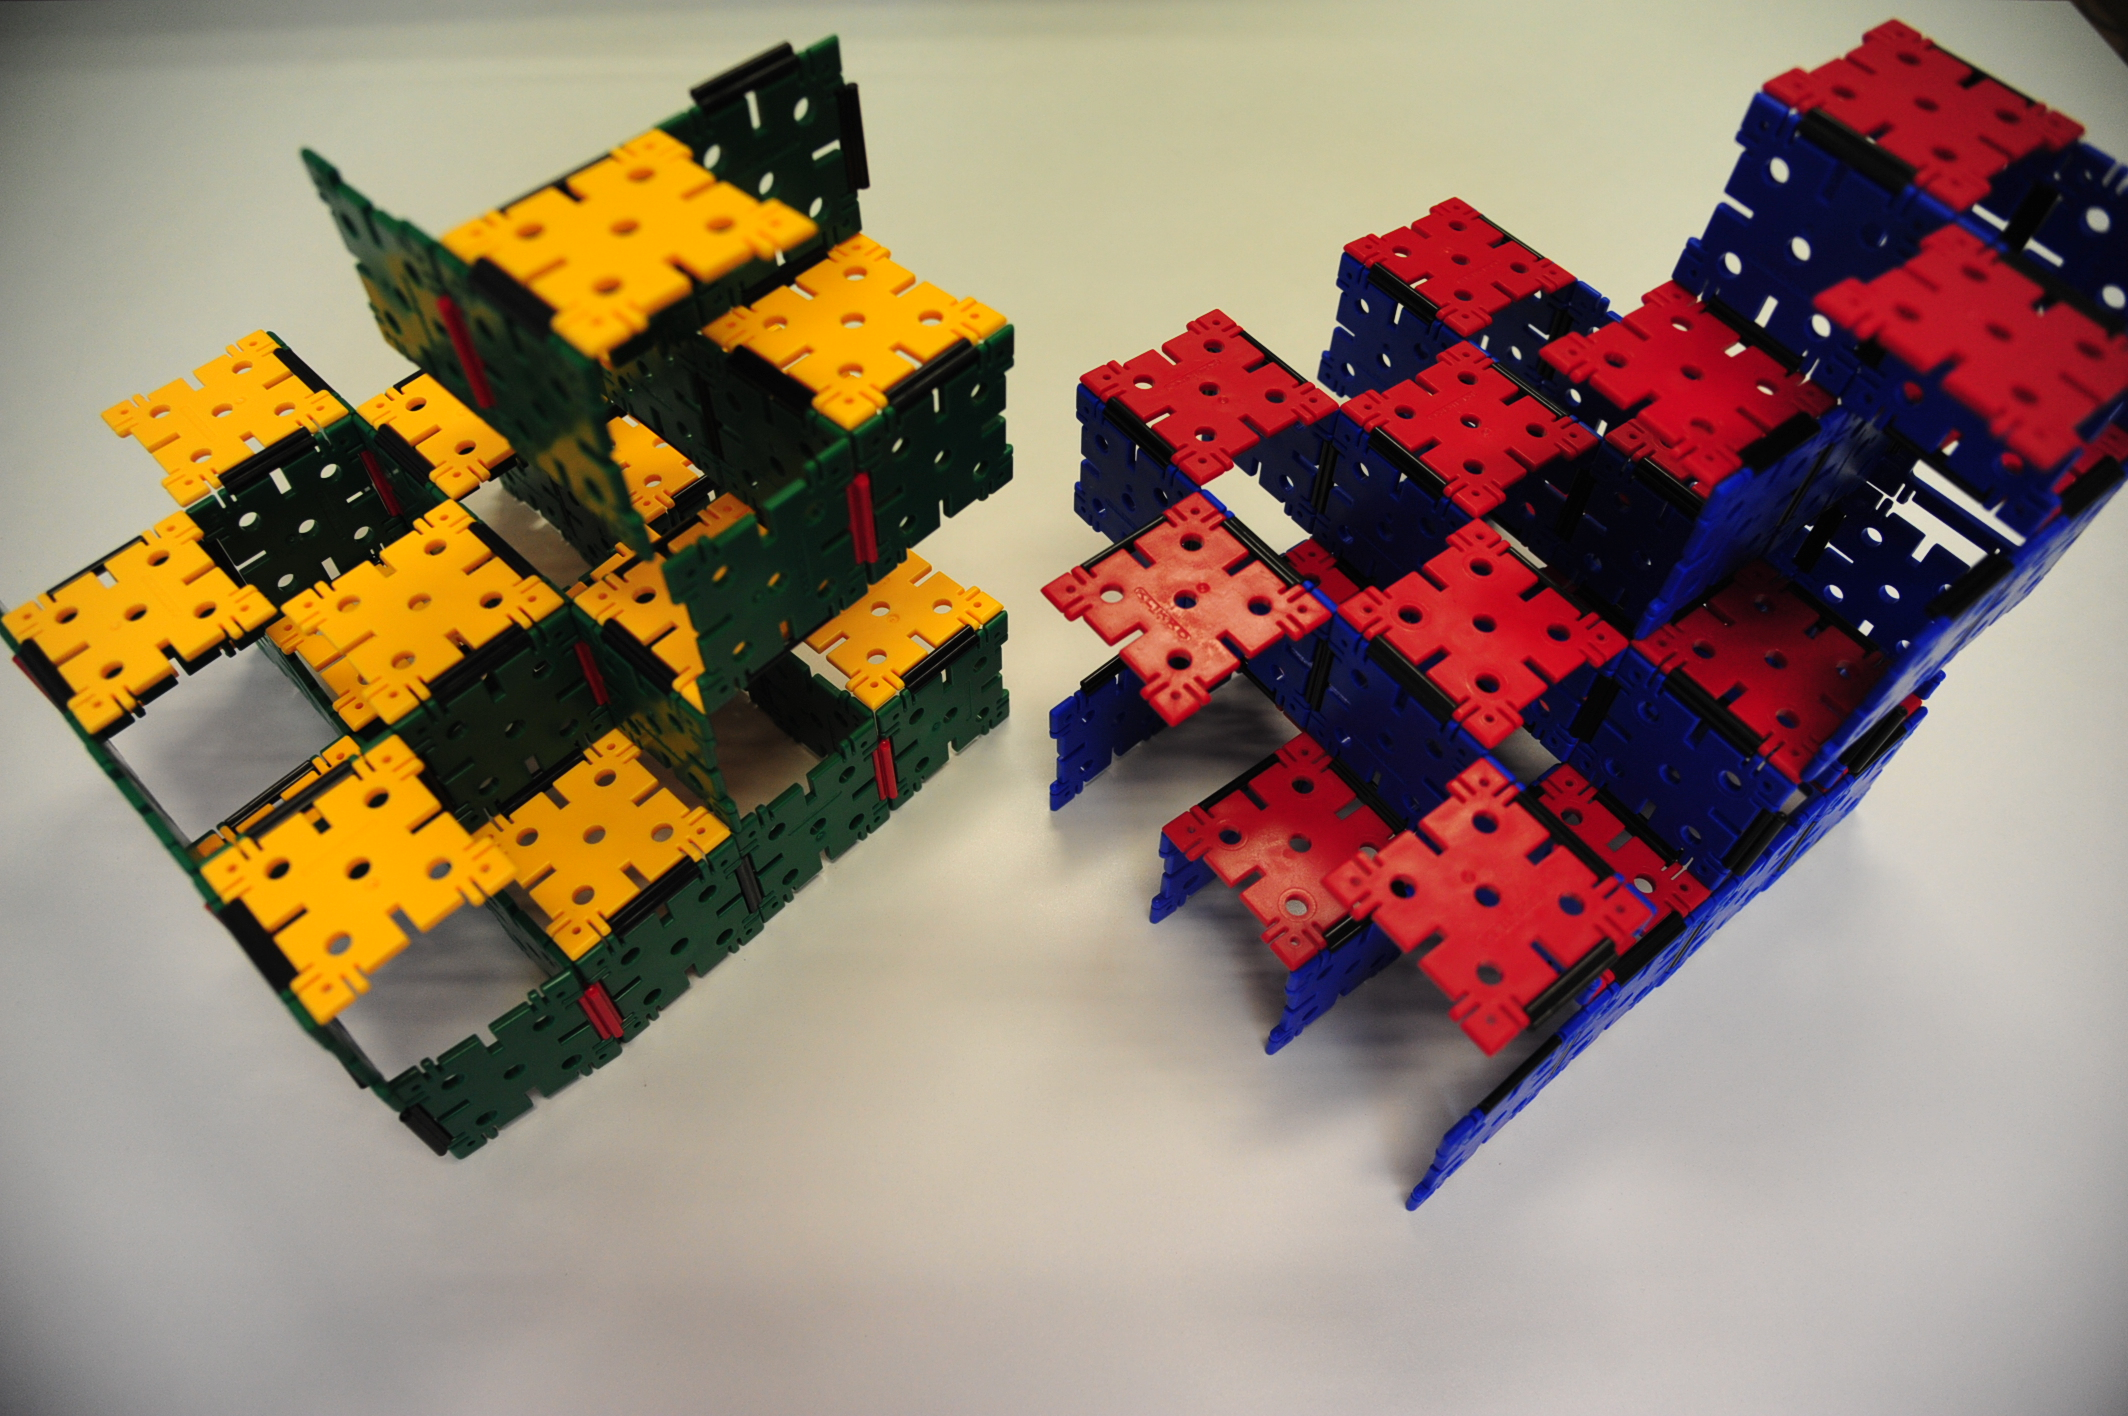
\includegraphics[height=4cm]{toys}
%		\end{center}
%	\end{column}
%	\begin{minipage}[t][0.5\textheight]{0.55\textwidth}
      \tableofcontents
%    \end{minipage}\hfill
%	\end{columns}
\end{frame}


\section{Introduction to Topological Crystalline States (TCSs)}

\begin{frame}
  \frametitle{Symmetry-Protected Topological (SPT) phases}
  \begin{itemize}
  \item Landau paragidm: phases are classified by symmetry breaking.
    \begin{center}
      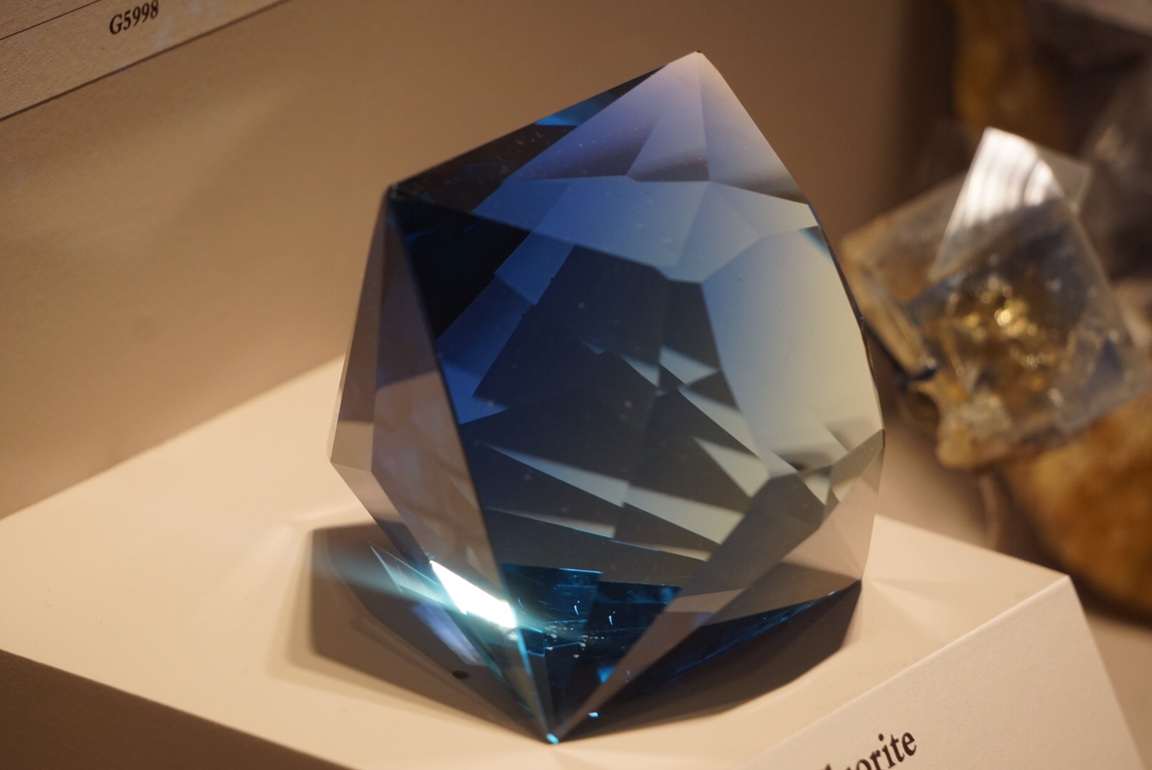
\includegraphics[height=1.5cm]{../resources/crystal}~~
      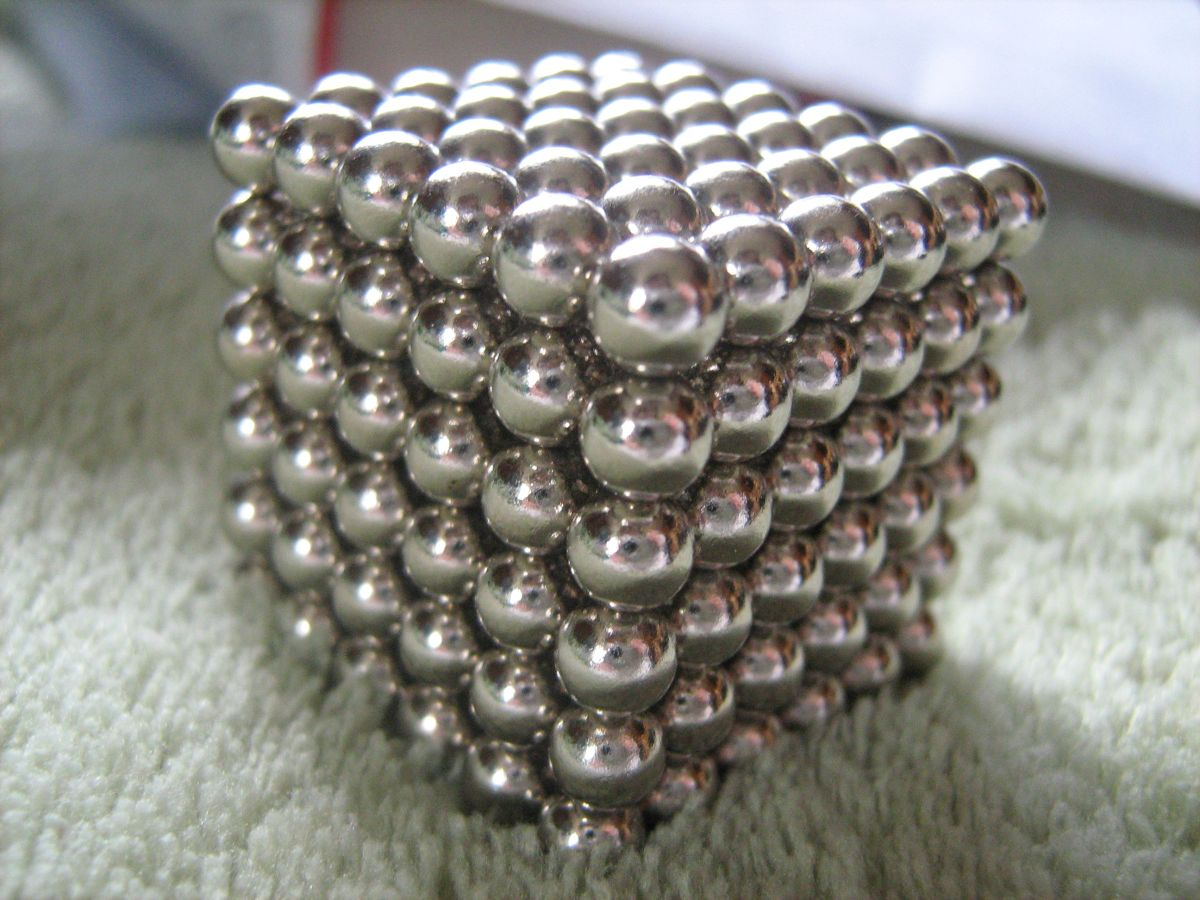
\includegraphics[height=1.5cm]{../resources/magnet}~~
      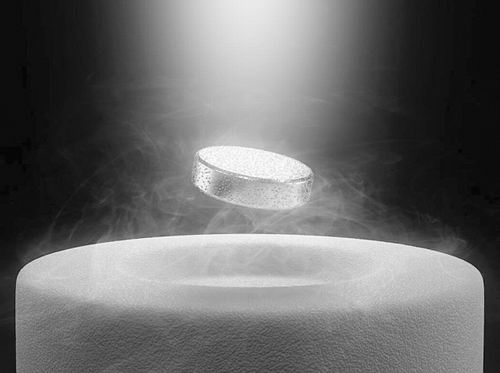
\includegraphics[height=1.5cm]{../resources/sc}
    \end{center}
  \item SPT: gapped topological phases beyond Landau paradiam.
  \item Gapped bulk : cannot be smoothly connected to a trivial state without closing gap or breaking symmetry.
  \item Symmetry-protected gapless surface states.
  \item Example: integer quantum Hall states; topological insulators.
    \begin{center}
      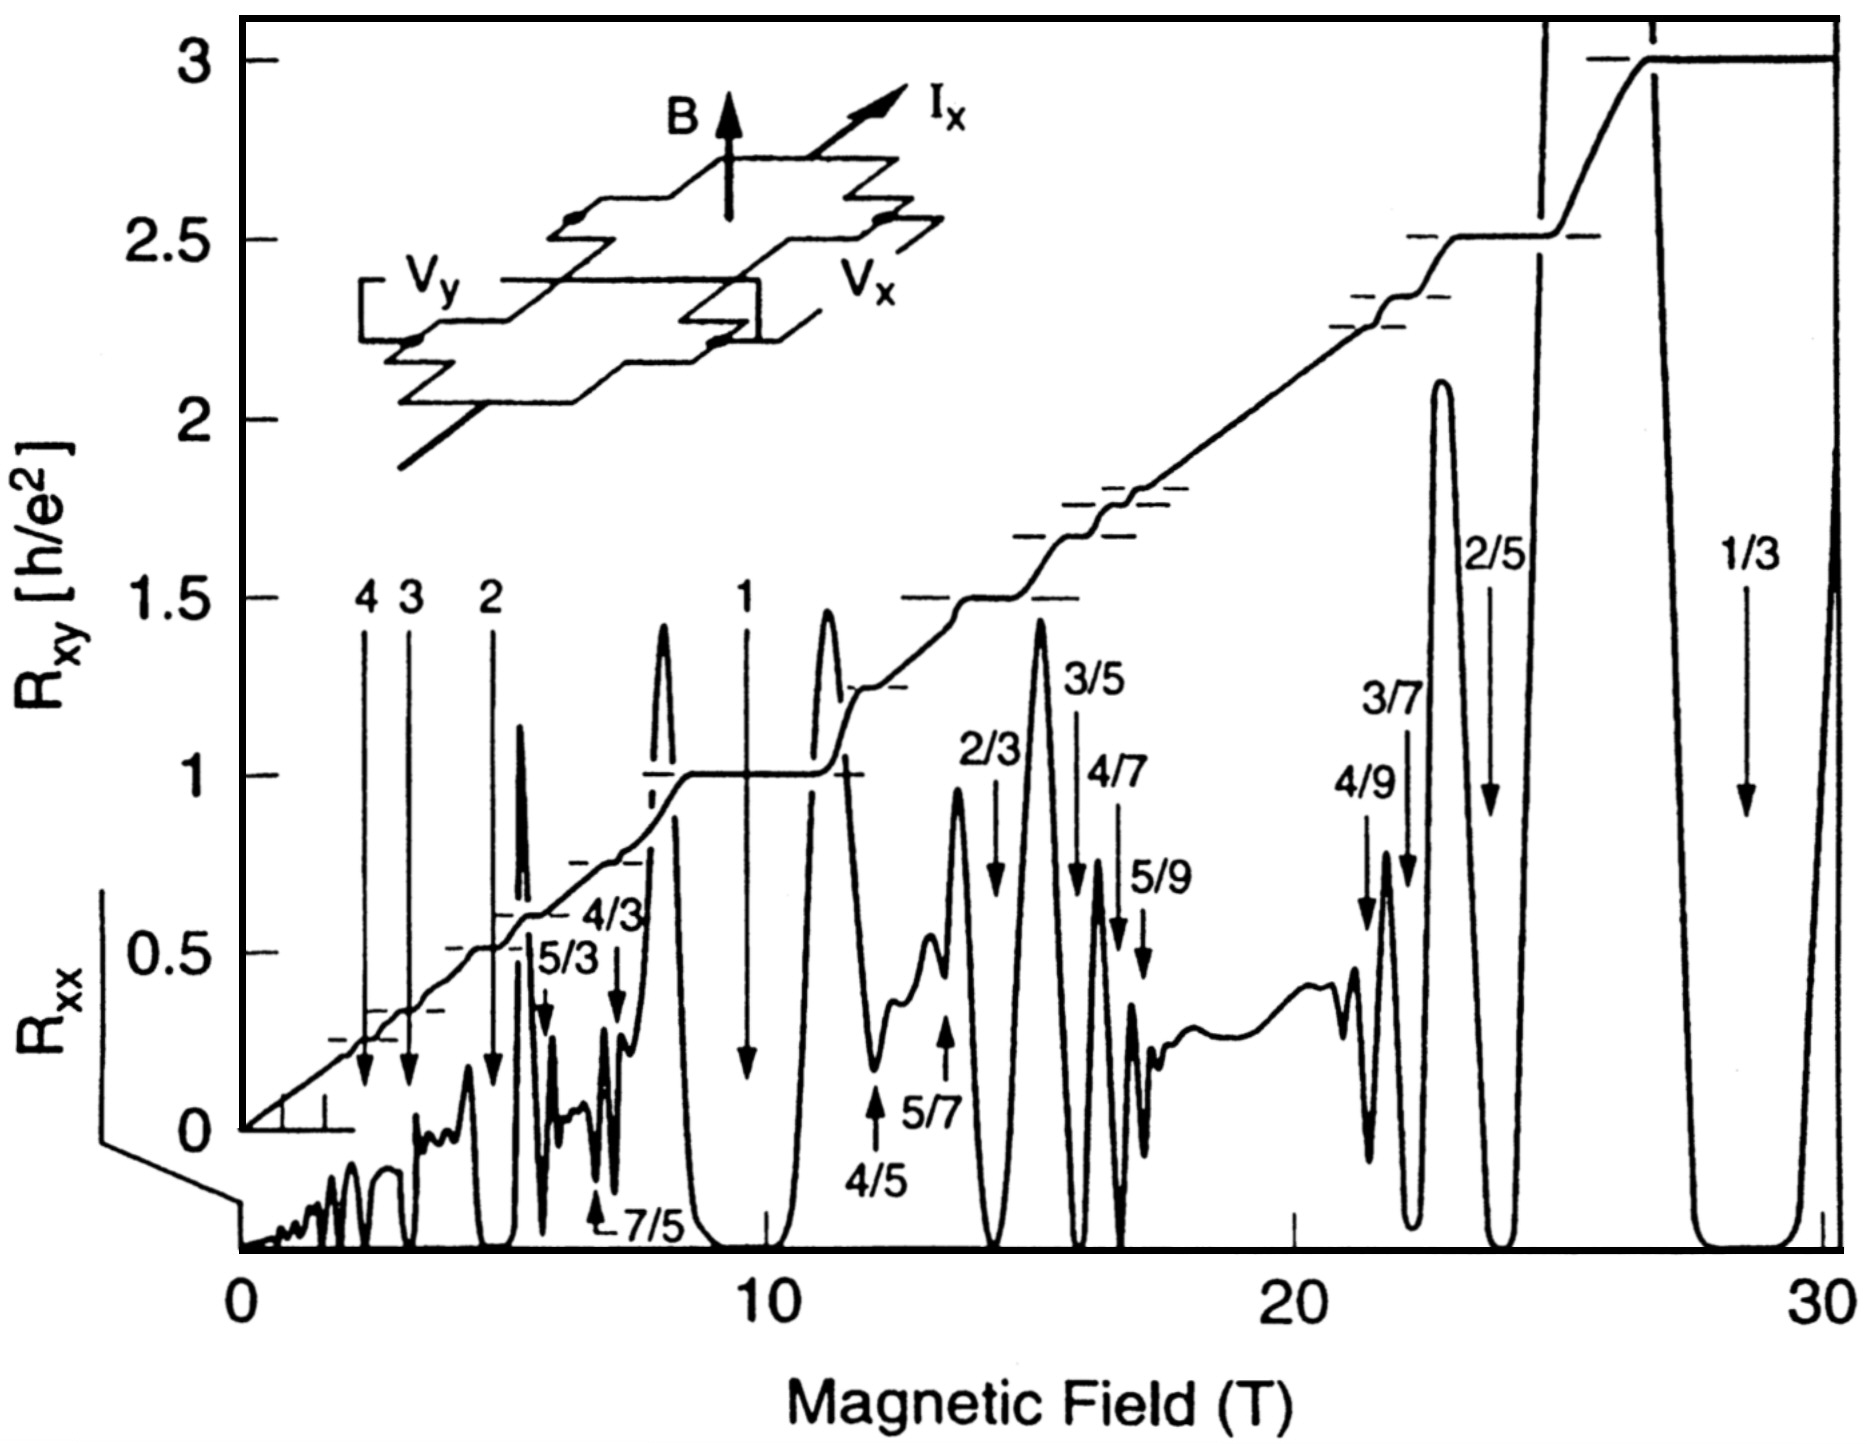
\includegraphics[height=2cm]{../resources/fqhe}~~
      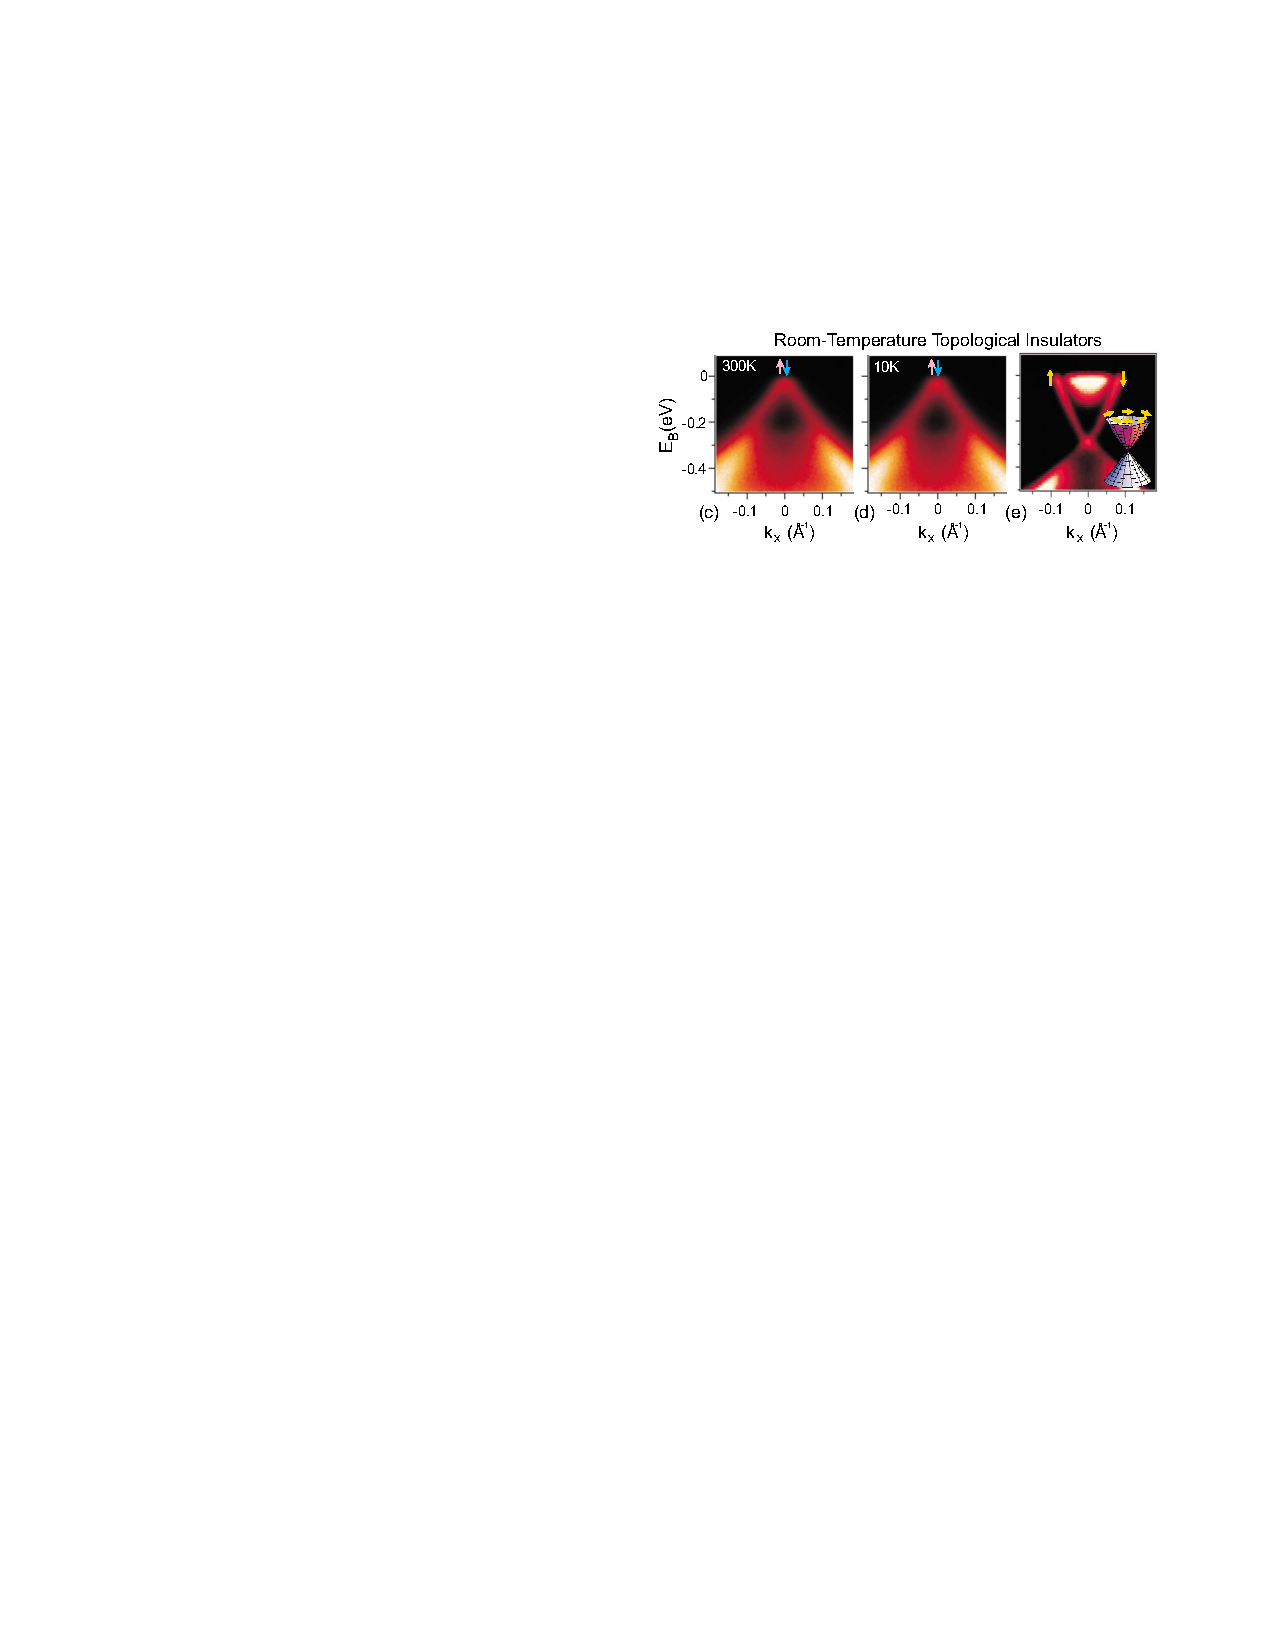
\includegraphics[height=2cm]{../spspt/ti_surface}
    \end{center}
  \end{itemize}
\end{frame}

\begin{frame}{Topological Crystaline States = Space-group SPT}
  \begin{itemize}
    \item Example: Topological Crystalline Insulators.
  \end{itemize}
  
\end{frame}

\begin{frame}
    \frametitle{Classification of Topological Crystaline States}
    \begin{itemize}
    \item Two approaches:
      \begin{enumerate}
      \item Thorngren and Else (2018): the crystalline equivalence principle
        \[SG\simeq G;\quad \Phi^d(SG)\simeq\Phi^d(G).\]
      \item Real-space recipes: Zhida Song, Chen Fang and YQ, Nat. Commun. (2020).\\
        \emph{Examples: mirror SPT, weak SPT (translation symmetry).}
        %\emph{Patch construction: Zhida Song, Shengjie Huang, YQ, Chen Fang and Michael Hermele, Sci. Adv. 5, eaax2007 (2019).}
      \end{enumerate}
    \item Application to free-fermion systems?
    \end{itemize}
    \begin{center}
    \begin{tikzpicture}[scale=.9]
    \fill [blue!20] (0,0)--(1,1)--(1,3)--(0,2)--(0,0);
    \draw (0,0)--(0,2)--(1,3);
    \draw (-1.5,0)--(1.5,0)--(1.5,2)--(-1.5,2)--(-1.5,0);
    \draw (1.5,0)--(2.5,1)--(2.5,3)--(1.5,2);
    \draw (2.5,3)--(-.5,3)--(-1.5,2);
    \end{tikzpicture}
    \hspace{2em}
    \begin{tikzpicture}[scale=.9]
    \fill [blue!40,opacity=.5] (0,0)--(1,1)--(1,3)--(0,2)--(0,0);
    \draw (0,0)--(0,2)--(1,3);
    \fill [blue!40,opacity=.5] (.5,0)--(1.5,1)--(1.5,3)--(0.5,2)--(0.5,0);
    \draw (.5,0)--(.5,2)--(1.5,3);
    \fill [blue!40,opacity=.5] (1,0)--(2,1)--(2,3)--(1,2)--(1,0);
    \draw (1,0)--(1,2)--(2,3);
    \fill [blue!40,opacity=.5] (-.5,0)--(.5,1)--(.5,3)--(-0.5,2)--(-0.5,0);
    \draw (-.5,0)--(-.5,2)--(.5,3);
    \fill [blue!40,opacity=.5] (-1,0)--(0,1)--(0,3)--(-1,2)--(-1,0);
    \draw (-1,0)--(-1,2)--(0,3);
    \draw (-1.5,0)--(1.5,0)--(1.5,2)--(-1.5,2)--(-1.5,0);
    \draw (1.5,0)--(2.5,1)--(2.5,3)--(1.5,2);
    \draw (2.5,3)--(-.5,3)--(-1.5,2);
    \end{tikzpicture}
    \end{center}
    \end{frame}
    
    \begin{frame}{Why Topological Crystaline States?}
      \begin{itemize}
        \item Crystalline symmetries are present in all solid-state materials.
        \item High-order boundary states: TCSs (excluding the Atomic Insulators) are a.k.a. High-Order Topological States.
        May be useful for storing quantum information.
      \end{itemize}
      \begin{center}
        \begin{tikzpicture} [scale=2]
          \fill [blue!50] (0,0)--(1,0)--(1.5,.5)--(1.5,1.5)--(0.5,1.5)--(0,1)--(0,0);
          \draw [thick,red] (0,0)--(1,0)--(1,1)--(0,1)--(0,0);
          \draw [thick,red] (1,0)--(1.5,.5)--(1.5,1.5)--(1,1);
          \draw [thick,red] (1.5,1.5)--(0.5,1.5)--(0,1);
          \draw [thick,red] (0,0)--(.5,.5)--(.5,1.5);
          \draw [thick,red](.5,.5)--(1.5,.5);
          \fill [red] (0,0) circle (2pt);
          \fill [red] (1,0) circle (2pt);
          \fill [red] (0,1) circle (2pt);
          \fill [red] (1,1) circle (2pt);
          \fill [red] (0.5,0.5) circle (2pt);
          \fill [red] (1.5,0.5) circle (2pt);
          \fill [red] (0.5,1.5) circle (2pt);
          \fill [red] (1.5,1.5) circle (2pt);
        \end{tikzpicture}      
      \end{center}
    \end{frame}
  \end{document}